\begin{figure}[h]
\centering
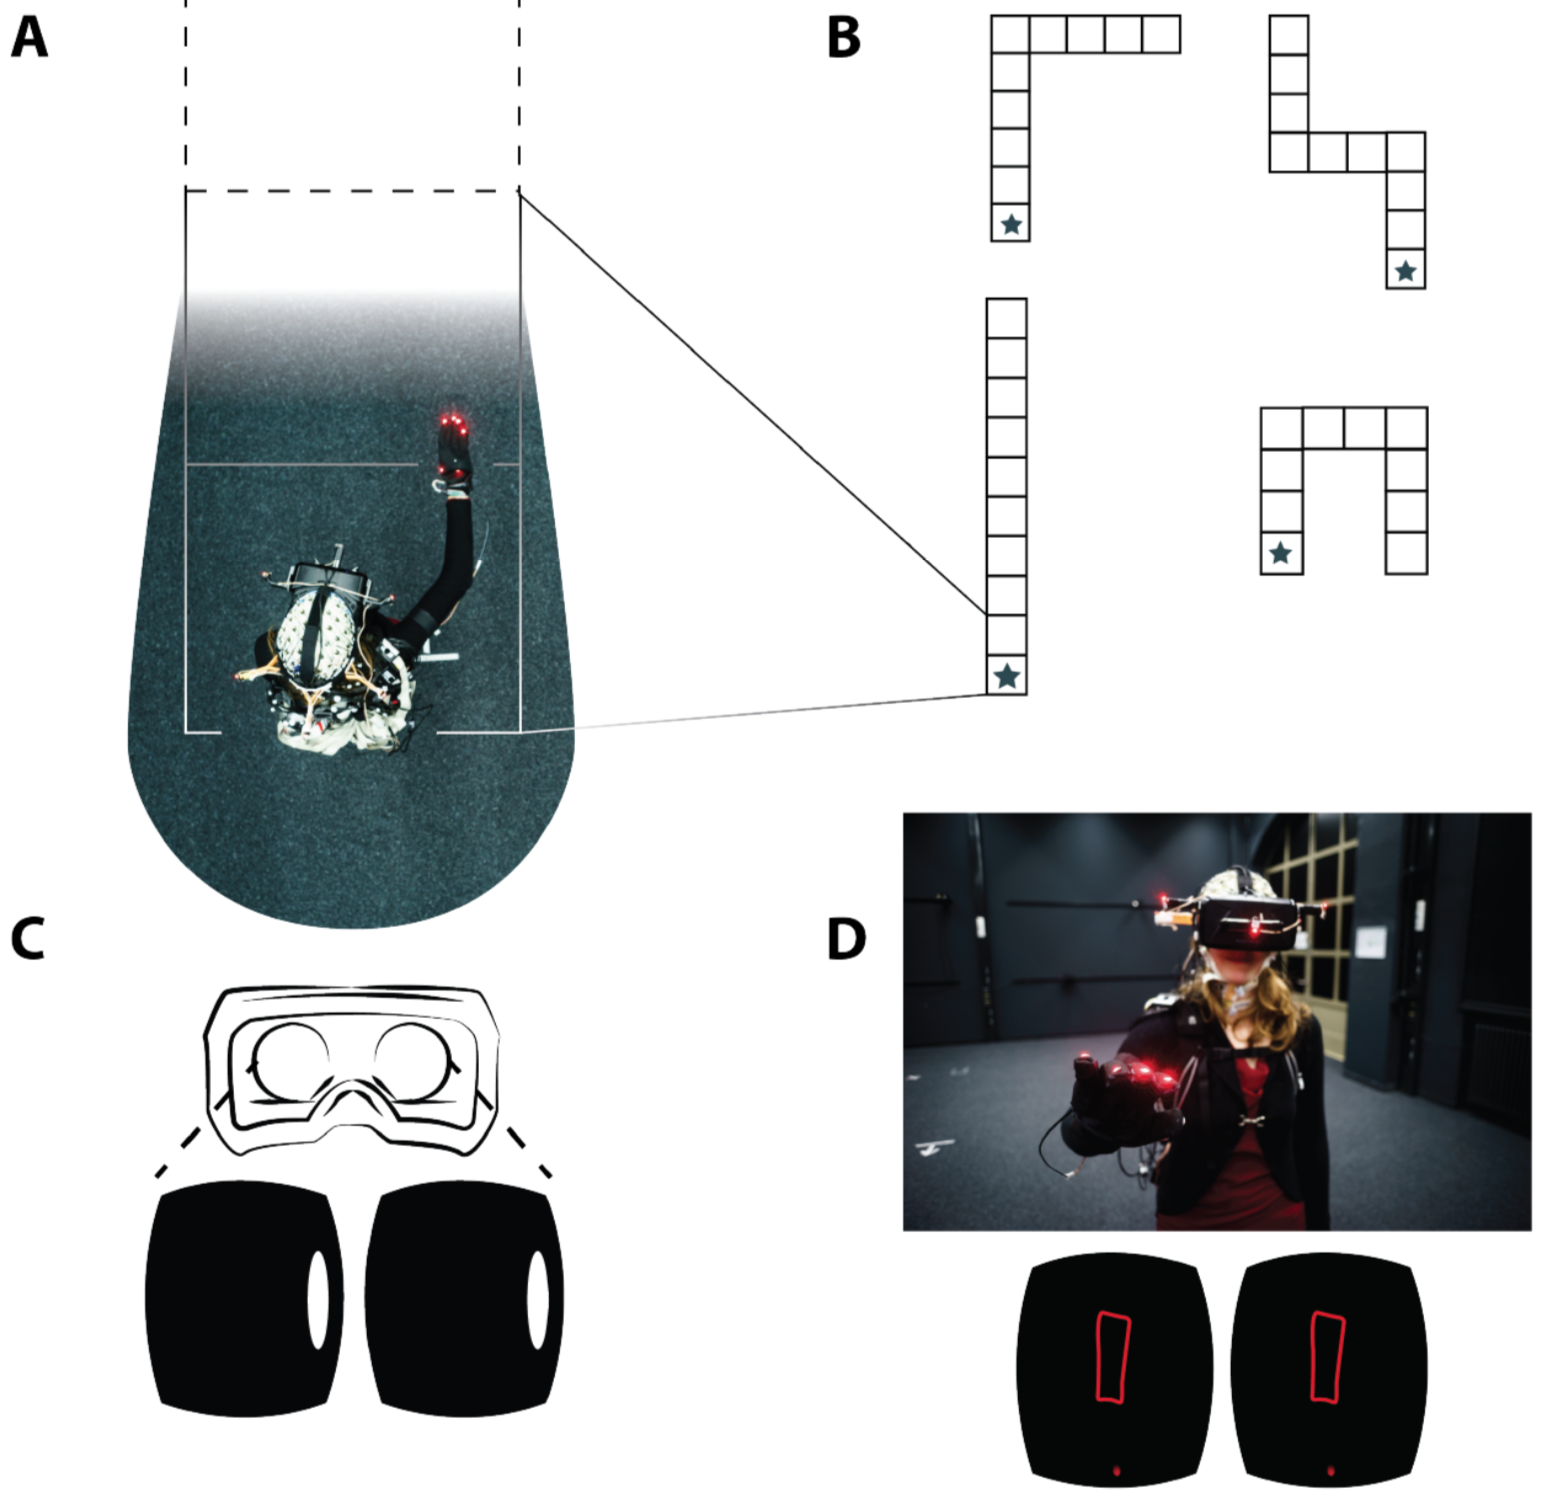
\includegraphics[width=\linewidth]{IMT_Task.png}
\vspace{0pt}
\caption{Invisible Maze Task, \textbf{A} Participant from a bird’s eye view. \textbf{B} Participants are instructed to explore four different mazes and return to the start. \textbf{C} First-person view in binocular ""VR optics"" of a wall touch. \textbf{D} Top: Participants draw a top-down view of the explored maze. Participant is equipped with 160 channels wireless EEG, head-mounted virtual reality goggles and LEDs for motion capture. Bottom: drawn sketch map. Find a detailed description in~\cite{Gehrke2018}}
\label{imt_task}
\end{figure}

\subsection{Summary and Hypotheses}
Here, we investigated the impact of experienced presence on spatial exploration behavior in the invisible maze task~\cite{Gehrke2018}. To address our motivation, we conducted the following two-step analysis. In a first step, we built a linear model to predict experienced presence given per participant descriptives. We were primarily interested to see how accurate presence can be predicted from broad knowledge of participant movement behavior. Additionally we considered a multitude of participant descriptives to derive a useful model. We reduced the model to a minimum of useful predictors so other researchers may easily reproduce our findings. In other words, we addressed how accurate subjectively reported presence may be predicted given a number of per participant descriptives.
In a second step, we increased the resolution of our analyses to specifically investigate ongoing motor behavior. Here, we analysed in detail whether participants movement behavior differed as a function of experienced presence and where it did so. To this end, we conducted mass-univariate pixel-by-pixel modeling of experienced presence on duration spent in a certain location and the number of wall touches elicited there, the simple where and what of participants actions.

% @Lukas: Should we then concentrate us on the term "place illusion" or generalize our claim to the general construct of presence? The subjective presence measure used (G1) is representing the sense of being in a place and therefore, more suitable as a metric for place illusion. If we do not want to go into much detail regarding the construct of presence, we can adapt the terminology of "the experience of presence" (also used by authors of IPQ) and in short only "presence". 

% @Sezen: no you are right, i do like place illusion much better. BTW there is a tracked changes and comment function in this overleaf now. Hit 'review' top right menu.

% @Lukas: Perfect, I tried half an hour ago without success :) Ill use from now on.